\documentclass[12pt, a4paper, oneside]{ctexart}
\usepackage{amsmath, amsthm, amssymb, graphicx}
\usepackage[bookmarks=true, colorlinks, citecolor=blue, linkcolor=black]{hyperref}
\usepackage[margin = 25mm]{geometry}
\usepackage{setspace}
\usepackage{listings}
\usepackage{ctex}
\usepackage{cite}
\usepackage{float}
\usepackage{xcolor}
\usepackage{amsmath}
\definecolor{codegreen}{rgb}{0,0.6,0}
\definecolor{codegray}{rgb}{0.5,0.5,0.5}
\definecolor{codepurple}{rgb}{0.58,0,0.82}
\definecolor{backcolour}{rgb}{0.95,0.95,0.92}

\lstdefinestyle{mystyle}{
    backgroundcolor=\color{backcolour},   
    commentstyle=\color{codegreen},
    keywordstyle=\color{magenta},
    numberstyle=\tiny\color{codegray},
    stringstyle=\color{codepurple},
    basicstyle=\ttfamily\footnotesize,
    breakatwhitespace=false,         
    breaklines=true,                 
    captionpos=b,                    
    keepspaces=true,                 
    numbers=left,                    
    numbersep=5pt,                  
    showspaces=false,                
    showstringspaces=false,
    showtabs=false,                  
    tabsize=2
}

\lstset{style=mystyle}


\title{Lennard-Jones势能下的液氩模拟暨GROMACS软件学习报告}
\date{\today}
\author{202011010101物理2001孙陶庵}
\begin{document}
\begin{spacing}{2.0}
\tableofcontents
\maketitle
\section{事前声明}
GROMACS是之前完全没有接触过的东西,连安装都不是执行档(exe),遇到了非常多的困难;我在网络上找到了马普所的Prof. Bert de Groot写得一篇文章\cite{NBS_2021},就是直接和这次大作业的主题对上的。
该文章的前半部分讲得是气体的拟合,后半部分讲得是液体部分的。因为网络上的教程太过于稀少(无论中英文),就算有,也是又臭又长的影片,根本无法在一周之内学习完然后完成报告,所以只能使用这位教授的源代码,只做学习之用绝无抄袭之意。
我以下这些东西基本都是使用这位教授的源代码,以作为学习之用,绝无抄袭之意图,但同时本文中讨论的部分以及分析结果的部分都是自己搜集资料查询并得出的结果。
使用软件:\\
1.GROMACS\\
2.Pymol\\
3.python
\section{Lennard-Jones势能模型}
$V(r)=4\epsilon\left[\left(\frac{\sigma}{r}\right)^{12}-\left(\frac{\sigma}{r}\right)^6\right]$
其中,$V(r) $表示两个粒子之间的势能,$\epsilon$表示势能的深度参数,$\sigma$表示粒子间的距离参数,r 表示两个粒子之间的距离。

模型的物理解释:
\\
1.斥力项:第一项$\left(\frac{\sigma}{r}\right)^{12}$表示斥力项,它随着粒子之间距离的减小而迅速增大。这一项源于泡利不相容原理,即两个粒子之间的电子云不能重叠。
当两个粒子靠得很近时,由于泡利不相容原理的限制,电子云之间的排斥力急剧增加,导致斥力项迅速增大,使得粒子之间发生排斥作用。
这一项的存在可以解释为什么物质的体积是有限的,因为当粒子之间的距离趋近于零时,斥力项趋近于正无穷大,使得粒子无法进一步靠近。\\
2.引力项:第二个项$\left(\frac{\sigma}{r}\right)^6$表示引力项,它随着粒子之间距离的减小而迅速减小。这一项源于分子之间的范德华力,即分子之间由于电荷分布产生的吸引力。
当两个粒子之间的距离较大时,引力项占主导地位,使得粒子之间发生吸引作用。然而,随着距离的减小,斥力项的贡献逐渐增大,抵消了引力项的作用,
导致势能逐渐减小。这一项的存在可以解释为什么物质在一定范围内具有吸引力,导致分子能够聚集成液体或固体的形态。

\section{问题}

使用gromacs在windows环境下进行液氩模拟实验\\
1.设定液氩系统的模拟参数。参数包括:氩原子数量,模拟箱的尺寸,温度,模拟总时间和步长等\\
2.使用Lennard-Jones势能描述氩原子的相互作用,进行液氩的分子动力学模拟\\
3.记录模拟过程中的数据,包括系统的能量温度压强等物理量的时间演化\\
4.分析结果,解释模拟结果的物理意义,并于理论预测结果相比较\\
\section{初始文件设置}
\subsection{设定拓扑文件}
\begin{lstlisting}[caption={argon.top}]
    [ defaults ]
; nbfunc        comb-rule       gen-pairs       fudgeLJ fudgeQQ
  1             1               no              1.0     1.0

[ atomtypes ]
AR  39.948    0.0   A     0.00622127     9.69576e-06

[ moleculetype ]
; molname       nrexcl
Ar              1

[ atoms ]
; id    at type res nr  residu name     at name  cg nr   charge
1       AR       1       Ar              Ar        1       0

[ system ]
; Name
Argon

[ molecules ]
; Compound        #mols
AR                216
\end{lstlisting}
其中[ atomtypes ]里面的A项(0.0后面0.00622127前面)即为Lennard-Jones势能在gromacs的代号
\subsection{设定结构文件}
总共219行的参数文件,参见附件
\subsection{设定分子动力学参数(mdp)}
\begin{lstlisting}[caption={94k.mdp}]
    ;
;	File 'mdout.mdp' was generated
;	By user: bert (1001)
;	On host: bertp3
;	At date: Sat Dec  4 13:41:42 2004
;

; VARIOUS PREPROCESSING OPTIONS
include                  = 
define                   = 

; RUN CONTROL PARAMETERS
integrator               = md
; Start time and timestep in ps
tinit                    = 0
dt                       = 0.002
nsteps                   = 500000
; For exact run continuation or redoing part of a run
init_step                = 0
; mode for center of mass motion removal
comm-mode                = Linear
; number of steps for center of mass motion removal
nstcomm                  = 1
; group(s) for center of mass motion removal
comm-grps                = 

; LANGEVIN DYNAMICS OPTIONS
; Temperature, friction coefficient (amu/ps) and random seed
bd-fric                  = 0
ld-seed                  = 1993

; ENERGY MINIMIZATION OPTIONS
; Force tolerance and initial step-size
emtol                    = 10
emstep                   = 0.01
; Max number of iterations in relax_shells
niter                    = 20
; Step size (1/ps^2) for minimization of flexible constraints
fcstep                   = 0
; Frequency of steepest descents steps when doing CG
nstcgsteep               = 1000
nbfgscorr                = 10

; OUTPUT CONTROL OPTIONS
; Output frequency for coords (x), velocities (v) and forces (f)
nstxout                  = 10000
nstvout                  = 10000
nstfout                  = 0
; Output frequency for energies to log file and energy file
nstlog                   = 100
nstcalcenergy            = 1
nstenergy                = 100
; Output frequency and precision for xtc file
nstxout-compressed       = 500
compressed-x-precision   = 1000
; This selects the subset of atoms for the xtc file. You can
; select multiple groups. By default all atoms will be written.
xtc-grps                 = 
; Selection of energy groups
energygrps               = System

; long-range cut-off for switched potentials
cutoff-scheme            = Verlet

; NEIGHBORSEARCHING PARAMETERS
; nblist update frequency
nstlist                  = 50
; Periodic boundary conditions: xyz (default), no (vacuum)
; or full (infinite systems only)
pbc                      = xyz
; nblist cut-off        
rlist                    = 0.85


; OPTIONS FOR ELECTROSTATICS AND VDW
; Method for doing electrostatics
coulombtype              = Cut-off
rcoulomb-switch          = 0
rcoulomb                 = 0.85
; Dielectric constant (DC) for cut-off or DC of reaction field
epsilon-r                = 1
; Method for doing Van der Waals
vdw-type                 = Cut-off
; cut-off lengths       
rvdw-switch              = 0
rvdw                     = 0.85
; Apply long range dispersion corrections for Energy and Pressure
DispCorr                 = Enerpres
; Extension of the potential lookup tables beyond the cut-off
table-extension          = 1
; Spacing for the PME/PPPM FFT grid
fourierspacing           = 0.12
; FFT grid size, when a value is 0 fourierspacing will be used
fourier_nx               = 0
fourier_ny               = 0
fourier_nz               = 0
; EWALD/PME/PPPM parameters
pme_order                = 4
ewald_rtol               = 1e-05
ewald_geometry           = 3d
epsilon_surface          = 0

; IMPLICIT SOLVENT (for use with Generalized Born electrostatics)
implicit_solvent         = No

; OPTIONS FOR WEAK COUPLING ALGORITHMS
; Temperature coupling  
Tcoupl                   = v-rescale
; Groups to couple separately
tc-grps                  = System
; Time constant (ps) and reference temperature (K)
tau_t                    = 0.1
ref_t                    = 94.4
; Pressure coupling     
Pcoupl                   = No
Pcoupltype               = isotropic
; Time constant (ps), compressibility (1/bar) and reference P (bar)
tau_p                    = 0.5
compressibility          = 4.5e-5
ref_p                    = 10.0

; SIMULATED ANNEALING  
; Type of annealing for each temperature group (no/single/periodic)
annealing                =  
; Number of time points to use for specifying annealing in each group
annealing_npoints        = 
; List of times at the annealing points for each group
annealing_time           = 
; Temp. at each annealing point, for each group.
annealing_temp           = 

; GENERATE VELOCITIES FOR STARTUP RUN
gen_vel                  = no
gen_temp                 = 100.0
gen_seed                 = 173529

; OPTIONS FOR BONDS    
constraints              = all-bonds
; Type of constraint algorithm
constraint-algorithm     = Lincs
; Do not constrain the start configuration
continuation             = no
; Use successive overrelaxation to reduce the number of shake iterations
Shake-SOR                = no
; Relative tolerance of shake
shake-tol                = 1e-04
; Highest order in the expansion of the constraint coupling matrix
lincs-order              = 4
; Number of iterations in the final step of LINCS. 1 is fine for
; normal simulations, but use 2 to conserve energy in NVE runs.
; For energy minimization with constraints it should be 4 to 8.
lincs-iter               = 1
; Lincs will write a warning to the stderr if in one step a bond
; rotates over more degrees than
lincs-warnangle          = 30
; Convert harmonic bonds to morse potentials
morse                    = no

; ENERGY GROUP EXCLUSIONS
; Pairs of energy groups for which all non-bonded interactions are excluded
energygrp_excl           = 

; NMR refinement stuff 
; Distance restraints type: No, Simple or Ensemble
disre                    = No
; Force weighting of pairs in one distance restraint: Conservative or Equal
disre-weighting          = Conservative
; Use sqrt of the time averaged times the instantaneous violation
disre-mixed              = no
disre-fc                 = 1000
disre-tau                = 0
; Output frequency for pair distances to energy file
nstdisreout              = 100
; Orientation restraints: No or Yes
orire                    = no
; Orientation restraints force constant and tau for time averaging
orire-fc                 = 0
orire-tau                = 0
orire-fitgrp             = 
; Output frequency for trace(SD) to energy file
nstorireout              = 100

; Free energy control stuff
free-energy              = no
init-lambda              = 0
delta-lambda             = 0
sc-alpha                 = 0
sc-sigma                 = 0.3

; Non-equilibrium MD stuff
acc-grps                 = 
accelerate               = 
freezegrps               = 
freezedim                = 
cos-acceleration         = 0

; Electric fields      
; Format is number of terms (int) and for all terms an amplitude (real)
; and a phase angle (real)
E-x                      = 
E-xt                     = 
E-y                      = 
E-yt                     = 
E-z                      = 
E-zt                     = 

; User defined thingies
user1-grps               = 
user2-grps               = 
userint1                 = 0
userint2                 = 0
userint3                 = 0
userint4                 = 0
userreal1                = 0
userreal2                = 0
userreal3                = 0
userreal4                = 0
\end{lstlisting}
包含初始条件及其它参数
\section{编译-结果-及分析}
分别输入以下命令:
\begin{lstlisting}
    gmx grompp -f 94k.mdp -c liquid.gro -p argon.top
    gmx mdrun -v -c liquid.pdb -nice 0
    gmx msd -s -o msd.xvg -f traj_comp.xtc -trestart 50 -b 100
\end{lstlisting}
并且设定完全后,会得到xvg档案,我们使用python分析画图
\begin{figure}[H]
    \begin{minipage}[t]{0.5\linewidth}
        \centering
        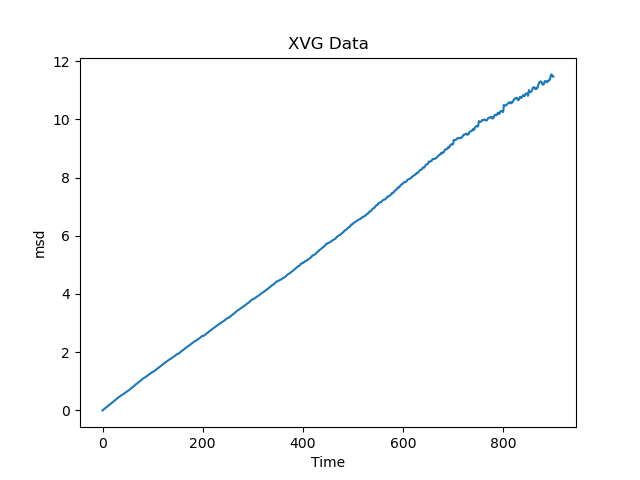
\includegraphics[scale=0.3]{msdxvg.png}
        \caption{结果}
        \label{fig:side:a}
      \end{minipage}%
      \begin{minipage}[t]{0.5\linewidth}
        \centering
        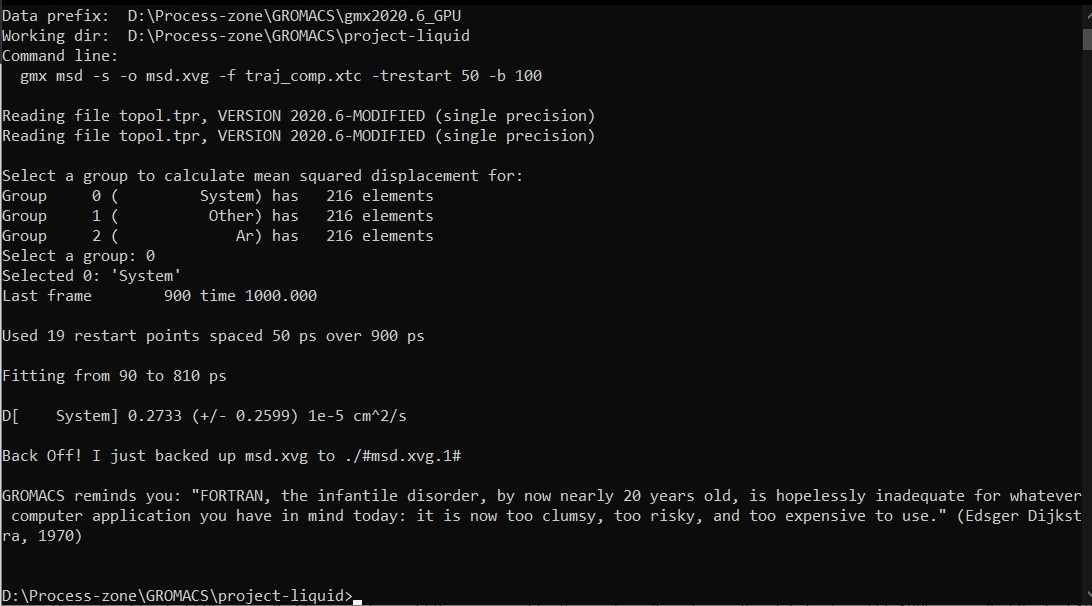
\includegraphics[scale=0.3]{msdxvgworking.jpg}
        \caption{得到扩散系数$2.1853\times 10^{-5}cm^2/s$}
        \label{fig:side:b}
      \end{minipage}
\end{figure}

\section{分子模拟}
\begin{lstlisting}
    wget http://www3.mpibpc.mpg.de/groups/de_groot/compbio1/p1/anneal2.mdp
    gmx grompp -f anneal2.mdp -c liquid.gro -p argon.top -maxwarn 1
    gmx mdrun -v -c anneal2.pdb -nice 0
\end{lstlisting}
以上指令用于跑(mdrun)出拟合档案liquid.gro(结构文件)及 traj\_comp.xtc(轨迹文件)
将以上这两个文件放在Pymol中打开后会得到一段分子振动的影片,并将其打印成GIF档(见附件)
\section{径向分布函数(RDF)分析}
RDF可以提供有关系统中粒子之间的距离分布信息。分析RDF可以确定粒子之间的最近邻距离、平均距离以及周期性结构(如晶体中的晶格常数)同时
在研究相变过程中也非常有用。相变通常涉及粒子的聚集或分散,以及结构的变化。通过监测RDF随温度、压力或其他条件的变化,可以探索相变过程中粒子的聚集行为。
接下来讨论如何使用rdf来分析:
\begin{figure}[H]
    \begin{minipage}[t]{0.5\linewidth}
        \centering
        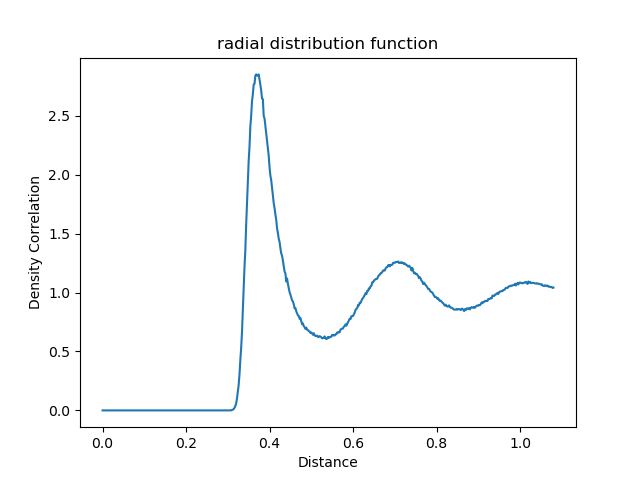
\includegraphics[scale=0.5]{radial distribution function.png}
        \caption{liquid}
        \label{fig:side:a}
      \end{minipage}%
      \begin{minipage}[t]{0.5\linewidth}
        \centering
        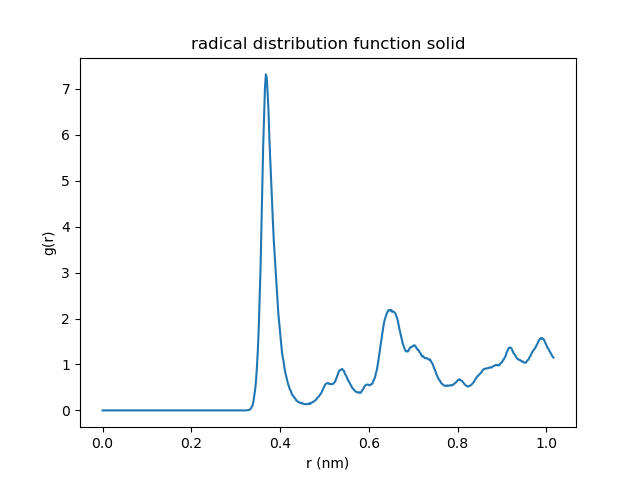
\includegraphics[scale=0.5]{radial distribution function solid.png}
        \caption{solid}
        \label{fig:side:b}
      \end{minipage}
\end{figure}


通过模拟液态氩和固态氩的系统,可以观察和比较两种相态的结构和性质。液态氩的原子会存在较大的自由度和较弱的相互作用,而固态氩的原子会排列成有序的晶格结构,并具有较强的相互作用。
固体部分在r=0.4 nm时达到了约7左右的极端值,而液体部分只有不到3。这说明在固体相中,在距离为0.4 nm的位置上,原子之间存在更强烈的相互作用或者更密集的排列。
这大概是因为固体和液体的结构差异。在固体中,原子通常排列成紧密的晶格结构,原子之间的相互作用力更强,因此在g(r)函数中会观察到较高的峰值。
而在液体中,原子之间的排列相对更为松散,相互作用力较弱,因此在g(r)函数中的峰值较低。
\begin{figure}[H]
	\centering
	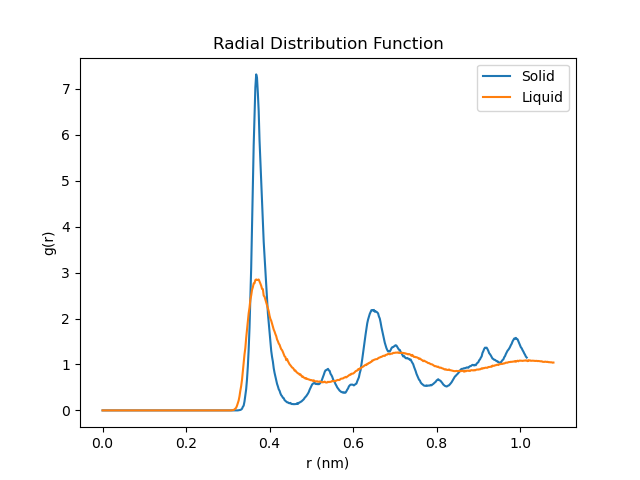
\includegraphics[width=8cm]{Radial Distribution Function2.png}
	\caption{all in one}
\end{figure}

\section{可以修改的参数并且与之而来的结果模拟及解释}

\end{spacing}{}
\bibliographystyle{IEEEtran}
\bibliography{6thre}

\end{document}